\documentclass{birkjour}

\usepackage{tikz}
\usepackage{graphicx}
\usepackage{hyperref}
\usepackage{algpseudocode}
\usepackage{graphicx}

\newtheorem{thm}{Theorem}[section]
\newtheorem{cor}[thm]{Corollary}
\newtheorem{lem}[thm]{Lemma}
\newtheorem{prop}[thm]{Proposition}
\theoremstyle{definition}
\newtheorem{defn}[thm]{Definition}
\theoremstyle{remark}
\newtheorem{rem}[thm]{Remark}
\newtheorem*{ex}{Example}
\numberwithin{equation}{section}

\newcommand{\R}{\mathbb{R}}
\newcommand{\B}{\mathbb{B}}
\newcommand{\G}{\mathbb{G}}
\newcommand{\V}{\mathbb{V}}
\newcommand{\gd}{\dot{g}}
\newcommand{\gh}{\hat{g}}
\newcommand{\Gd}{\dot{G}}
\newcommand{\Gh}{\hat{G}}
\newcommand{\nvai}{\infty}
\newcommand{\nvao}{o}
\newcommand{\grade}{\mbox{grade}}

%\received{}\accepted{}

\begin{document}

\title{An Introduction To Geometric Sets}

\author{Spencer T. Parkin}
\address{102 W. 500 S., \\
Salt Lake City, UT  84101} \email{spencerparkin@outlook.com}

%\subjclass{Primary 14J70; Secondary 14J29}

\dedicatory{To my dear wife Melinda.}

\begin{abstract}
A generalized model of geometry based upon the idea of using blades of a geometric algebra
as representatives of geometry is developed.  Similar to the idea of an algebraic set, the main object of study
becomes the notion of a geometric set.  Results about geometric sets are obtained, and their implications discussed.
Being a generalization, results obtained are immediately applicable to well-known models of geometry,
including the homogeneous and conformal models, as well as any specific future model that falls
under the generalization.
\end{abstract}

\keywords{Geometric Algebra, Model Of Geometry, Geometric Set}

\maketitle

\section{Introduction}

This paper studies a generalization of well-known models of geometry.
Specific examples include the homogeneous and conformal models (see \cite{Dorst07,Hestenes01,Lasenby04})
which have received much attention in recent years.

\subsection{Motivation}

Seeing a great deal of commonality between various models of geometry based upon
geometric algebra, a formal treatment of the subject deserves to be given in an abstract
setting in much the same way that, for example, abstract algebra provides such a setting
in which algebraic sets generated by ideals of a polynomial ring can be studied.
Readers familiar with algebraic geometry will no-doubt recognize at least some small overlap
between that subject and the subject of this paper.  For example, it will be seen
that in some cases, geometric sets are algebraic sets.

Another reason for investigating a generalized model is that it may provide enough theory that
we can actually make practical use out of a specific instance of the model that, for example,
uses blades to represent the quadrics.  It is not hard to find blades of a geometric algebra that
represent quadric surfaces, but it is hard to see how one can make any practical use out of such a model.

\subsection{Conventions}

This paper uses capital letters $A,B,C$ to denote blades of various grades,
while using lower case letters $a,b,c$ to denote vectors, unless stated otherwise.  Scalars are written
using Greek letters $\alpha,\beta,\gamma$.  Grades of blades $A,B,C$ are usually
denoted by lower case letters $r,s,t$, respectively, unless stated otherwise.  Lower case letters $i,j,k$ are
used as indices.  Capital letters $R,S,T$
are used to denote subsets of interest of $n$-dimensional euclidean space $\R^n$.
Lower case letters $x,y,z$ are reserved for denoting points taken from $\R^n$.  We
let $P(\R^n)$ denote the power set of $\R^n$.
We will use $\G$ to denote our geometric algebra, and $\V$ to denote an $m$-dimensional vector
space generating it.  $\B$ will denote the set of all blades taken from $\G$.  The
scalars of $\V$, and therefore $\G$, are taken from the field of real numbers $\R$.
The capital letter $I$ will be used to denote the unit pseudo-scalar of $\G$.  We assume
that $I$ is invertible with respect to the geometric product.  Furthermore, we'll assume, without
loss of generality, that $I^{-1}=-I$.

We will let the geometric product take precedence over the inner and outer products,
and the outer product take precedence over the inner product.

No specific signature of our geometric algebra $\G$ is assumed in this paper unless
one is given in a special case.

At times a blade $A$ may be referred to as a subspace.  The notion of blades as being
representatives of subspaces of $\V$ is a common practice and is employed throughout this paper.
It may also be said that a blade $A$ is a subspace of some other blade $B$; in which case,
it can be understood that for all vectors $a\in\V$ such that $a\wedge A=0$, we have $a\wedge B=0$.

\section{Preliminaries}

The results of this paper will depend upon the following preliminary material.
If desired, the reader is welcome to skip this material and refer back to it only as needed.

\subsection{Identities}

Given a vector $a\in\V$ and a blade $A\in\B$, central to all of geometric algebra is the identity
\begin{equation}\label{equ_vec_blade_geo_prod}
aA = a\cdot A + a\wedge A.
\end{equation}
The inner and outer products of \eqref{equ_vec_blade_geo_prod} may be written in terms
of the geometric product as
\begin{align}
a\wedge A &= \frac{1}{2}\left(aA + (-1)^rAa\right),\label{equ_vec_blade_outer_prod} \\
a\cdot A &= \frac{1}{2}\left(aA - (-1)^rAa\right),\label{equ_vec_blade_inner_prod}
\end{align}
where $r=\grade(A)$.  Then, realizing that $m=\grade(I)$, and that by \eqref{equ_vec_blade_geo_prod},
we have $aI=a\cdot I$, we can use equation \eqref{equ_vec_blade_inner_prod} to establish the
commutativity of vectors in $\V$ with the unit pseudo-scalar $I$ as
\begin{equation}\label{equ_blade_psuedo_scalar_commutativity}
aI = -(-1)^mIa.
\end{equation}
Using equation \eqref{equ_blade_psuedo_scalar_commutativity} in conjunction with equation \eqref{equ_vec_blade_inner_prod},
we find that
\begin{equation}\label{equ_vec_blade_inner_prod_dual}
(a\cdot A)I=a\wedge AI.
\end{equation}
(In verifying this identity, it helps to realize that for any integer $r$, we have $(-1)^r=(-1)^{-r}$.)
Replacing $A$ in equation \eqref{equ_vec_blade_inner_prod_dual} with $AI$, we find that
\begin{equation}\label{equ_vec_blade_outer_prod_dual}
(a\wedge A)I=a\cdot AI.
\end{equation}

Referring back to equation \eqref{equ_vec_blade_inner_prod}, another important formulation of the inner product between a vector and a blade
is given by
\begin{equation}\label{equ_vec_blade_inner_prod_series}
a\cdot A=-\sum_{i=1}^r(-1)^i(a\cdot a_i)A_i,
\end{equation}
where $A$ is factored as $\bigwedge_{i=1}^r a_i$, and we define $A_i$ as
\begin{equation}\label{equ_A_i}
A_i=\bigwedge_{\substack{j=1\\j\neq i}}^r a_i.
\end{equation}
This leads to the following recursive formulation.
\begin{equation}
a\cdot A = (a\cdot a_1)A_1-a_1\wedge(a\cdot A_1)
\end{equation}
If a blade $B\in\B$ has grade $s$ and factorization $\bigwedge_{i=1}^s b_i$, then we can express
the product $A\cdot B$ recursively as
\begin{equation}
A\cdot B = \left\{\begin{array}{ll}
A_r\cdot(a_r\cdot B) & \mbox{if $r\leq s$,} \\
(A\cdot b_1)\cdot B_1 & \mbox{if $r\geq s$.}
\end{array}\right.
\end{equation}

\subsection{Lemmas}

The following lemmas will become instrumental in the remainder of this paper.

\begin{lem}[Found Factorization Of Blade]\label{lem_desired_blade_factorization}
If $A\in\B$ is a non-zero blade of grade $r>0$ and $\{c_i\}_{i=1}^r$ is a set
of $r$ linearly independent vectors such that for all $c\in\{c_i\}_{i=1}^r$, we have
$c\wedge A=0$, then there exists a scalar $\beta\in\R$ such that
\begin{equation}\label{equ_desired_blade_factorization}
A = \beta C,
\end{equation}
where the $r$-blade $C$ is given by
\begin{equation}
C=\bigwedge_{i=1}^r c_i.
\end{equation}
\end{lem}
\begin{proof}
Letting $\bigwedge_{i=1}^r a_i$ be a factorization of the $r$-blade $A$, it is clear
that if $c_i\wedge A=0$, then there exists a set of $r$ scalars $\{\gamma_{i,j}\}_{j=1}^r$
such that
\begin{equation}\label{equ_c_i}
c_i=\sum_{j=1}^r\gamma_{i,j}a_j.
\end{equation}
We then have
\begin{equation}
\bigwedge_{i=1}^r c_i=(\det M)\bigwedge_{i=1}^r a_i,
\end{equation}
where the $r\times r$ matrix $M$ is given by
\begin{equation}
M = \left[\begin{array}{cccc}
\gamma_{1,1} & \gamma_{1,2} & \dots & \gamma_{1,r} \\
\gamma_{2,1} & \gamma_{2,2} & \dots & \gamma_{2,r} \\
\vdots & \vdots & \ddots & \vdots \\
\gamma_{r,1} & \gamma_{r,2} & \dots & \gamma_{r,r}
\end{array}\right].
\end{equation}
Now since $\{c_i\}_{i=1}^r$ is a linearly independent set of vectors,
$\det M\neq 0$, and we may choose $\beta=(\det M)^{-1}$ and
equation \eqref{equ_desired_blade_factorization} now holds.
\end{proof}

Our next lemma is a generalization of Lemma~\ref{lem_desired_blade_factorization}.

\begin{lem}[Found Partial/Full Factorization Of Blade]\label{lem_desired_partial_blade_factorization}
If $A\in\B$ is a non-zero blade of grade $r>0$ and $\{c_i\}_{i=1}^t$ is a set of $t\leq r$ linearly
independent vectors such that for all $c\in\{c_i\}_{i=1}^t$, we have $c\wedge A=0$, then there
exists a blade $B\in\B$ of grade $r-t$ such that
\begin{equation}\label{equ_desired_partial_blade_factorization}
A=B\wedge C,
\end{equation}
where $C$ is a $t$-blade given by
\begin{equation}
C = \bigwedge_{i=1}^t c_i.
\end{equation}
\end{lem}
\begin{proof}
The case of $t=r$ being handled by Lemma~\ref{lem_desired_blade_factorization}, and the
case of $r=1$ being trivial, we may assume that $0<t<r$.  Then, letting $\bigwedge_{i=1}^r a_i$
be a factorization of the $r$-blade $A$, it is clear that if $c_i\wedge A=0$, then there exists a
set of $r$ scalars $\{\gamma_{i,j}\}_{j=1}^r$ such that equation \eqref{equ_c_i} again holds.
Furthermore, we can assume, without loss of generality, that for each $c_i$, $\gamma_{i,i}\neq 0$.
We then have
\begin{equation}
\bigwedge_{i=1}^t c_i = \gamma\bigwedge_{i=1}^t a_i + Q,
\end{equation}
where $\gamma=\prod_{i=1}^t\gamma_{i,i}$ and $Q$ represents the remaining terms in the
expansion of $C$.  Letting
\begin{equation}
B=(-1)^{t(r-t)}\gamma^{-1}\bigwedge_{i=t+1}^r a_i,
\end{equation}
it follows now that equation \eqref{equ_desired_partial_blade_factorization} holds, since $B\wedge Q=0$.
\end{proof}

% may want to note that 0-blades in outer, inner and geometric products reduce to scalar-blade product

\begin{lem}\label{lem_lin_indep_blades}
For a non-zero $r$-blade $A$ factored as $\bigwedge_{i=1}^r a_i$, the set of
$(r-1)$-blades $\{A_i\}_{i=1}^r$, (see equation \eqref{equ_A_i}), is linearly independent.
\end{lem}
\begin{proof}
Suppose there exists a non-trivial set of $r$ scalars $\{\alpha_i\}_{i=1}^r$
such that $0 = \sum_{i=1}^r\alpha_i A_i$.
Then, without loss of generality, suppose that $\alpha_r\neq 0$, and rearrange
our equation as $-\alpha_rA_r=\sum_{i=1}^{r-1}\alpha_iA_i$.  Now notice
that while $a_r\wedge-\alpha_rA_r\neq 0$, we have $a_r\wedge\sum_{i=1}^{r-1}\alpha_iA_i=0$,
which is a contradiction.
\end{proof}

Note that a perhaps more elegant proof of Lemma~\ref{lem_lin_indep_blades} could have been given
under the assumption
of a euclidean signature; in which case, the Gram-Schmidt orthogonalization process would have
allowed us to choose, without loss of generality, an orthogonal factorization of the blade $A$.
Doing so, $A$ becomes the versor\footnote{Recall that a versor is any multivector that can
be written as the geometric product of one or more invertible vectors.} $\prod_{i=1}^r a_i$, and we may write
\begin{equation}\label{equ_elegant_proof_of_A_i_lin_indep}
0 = \sum_{i=1}^r \alpha_iA_i \iff
0=\left(\sum_{i=1}^r\alpha_iA_i\right)A = -\sum_{i=1}^r(-1)^{r-i}A_i^2\alpha_ia_i.
\end{equation}
The use of equation \eqref{equ_elegant_proof_of_A_i_lin_indep} would depend, in part, upon Lemma~\ref{lem_zero_prod_property} to follow.

\begin{lem}[The Zero Product Property]\label{lem_zero_prod_property}
For any two blades $A,B\in\B$ of grades $r$ and $s$, respectively, if $AB=0$ and at least one of $A$ and $B$
is invertible, then at least one of $A$ and $B$ is zero.
\end{lem}
\begin{proof}
Without loss of generality, suppose $B^{-1}$ exists.  We then see that
\begin{equation}
A=ABB^{-1}=0B^{-1}=0.
\end{equation}
\end{proof}

Notice the requirement here of Lemma~\ref{lem_zero_prod_property} that at least one of $A$ and $B$ be invertible.
This requirement comes about in consideration of the square of a non-zero null-vector.

\section{Results}

\subsection{Foundation}

Our discussion begins with a non-zero, undefined function $p:\R^n\to\V$.\footnote{By definition, a function is well-defined even if it is left unspecified.}
By leaving this function undefined, the results to follow generalize to the homogeneous model, conformal model,
and any other model of geometry that is based upon the use of blades as representatives of geometry in the
following manner.\footnote{For example, if we let
\begin{equation}\label{equ_p_conformal}
p(x)=\nvao+x+\frac{1}{2}x^2\nvai,
\end{equation}
we get the conformal model,
but by leaving our function $p:\R^n\to\V$ unspecified, we work in a generalization of which the conformal model
is simply a special case.}

\begin{defn}[Direct And Dual Representation]\label{def_gh_and_gd}
For the two functions $\gh:\B\to P(\R^n)$ and $\gd:\B\to P(\R^n)$, given by
\begin{align}
\gh(A) &= \{x\in\R^n|p(x)\wedge A=0\},\\
\gd(A) &= \{x\in\R^n|p(x)\cdot A=0\},
\end{align}
we say that $A$ directly represents the set of points $\gh(A)$ and
dually represents the set of points $\gd(A)$.\footnote{In the conformal model, since
$p(\R^n)$ is the set of all null-vectors taken from $\V$, $p(\gh(A))$ is the outer product
null-space of $A$, and $p(\gd(A))$ is the inner product null-space of $A$.}
\end{defn}

From Definition~\ref{def_gh_and_gd} it is important to take away the realization that a given blade $A\in\B$
represents two subsets of $\R^n$ simultaneously; namely, $\gh(A)$ and $\gd(A)$.  Which we choose
to think of $A$ as being a representative of at any given time is completely arbitrary.

It should also be clear from Definition~\ref{def_gh_and_gd} that the subset of $\R^n$ represented by a
blade $A$, (directly or dually), remains invariant under any non-zero scaling of the blade $A$.

Note that by Lemma~\ref{lem_dual_relationship_in_rep} (not yet given), we might
have also said that $A$ indirectly represents the
set $\gd(A)$, but as this lemma also shows, to say that it dually represents this set is equally
as reasonable.

At last, now enters this paper's object of study: the {\it geometric set}.

\begin{defn}[Geometric Set]\label{def_geo_set}
A subset $R\subset\R^n$ for which there exists a blade $A\in\B$ such that $\gh(A)=R$ is what
we'll refer to as a {\it geometric set}.
\end{defn}

In the course of our study, we will find significant the following concept of {\it irreducibility}.

\begin{defn}[Irreducible/Reducible Blade]\label{def_irreducible_blade}
Given an $r$-blade $A\in\B$, if there does not exist an $s$-blade $B\in\B$ with $s<r$
such that $\gh(A)=\gh(B)$, then $A$ is what we'll refer to as an {\it irreducible} blade.
A blade that is not irreducible is referred to as {\it reducible}.
\end{defn}

\subsection{Developments}

Having given the definitions in the previous section, we may now focus on the results that follow
from these definitions.

\subsubsection{Representation}

Our initial developments reveal results about the representations of geometric sets.

\begin{lem}[Dual Relationship Between Representations]\label{lem_dual_relationship_in_rep}
For any geometric set $R\subset\R^n$, if $A\in\B$ is a blade such that $\gh(A)=R$,
then $\gd(AI)=R$, and similarly, if $A\in\B$ is a blade such that $\gd(A)=R$, then $\gh(AI)=R$.
\end{lem}
\begin{proof}
By the identity of equation \eqref{equ_vec_blade_outer_prod_dual}, and Lemma~\ref{lem_zero_prod_property},
the first of these two latter statements is proven by
\begin{equation}
0=p(x)\wedge A=-(p(x)\cdot AI)I\iff p(x)\cdot AI=0,
\end{equation}
while the second, by the identity of equation \eqref{equ_vec_blade_inner_prod_dual},
and again Lemma~\ref{lem_zero_prod_property}, is proven by
\begin{equation}
p(x)\cdot A=0\iff 0=(p(x)\cdot A)I=p(x)\wedge AI.
\end{equation}
\end{proof}

In other words, Lemma~\ref{lem_dual_relationship_in_rep} is telling us that for a single given geometric set, the
algebraic relationship between a blade directly (dually) representative of that set,
and a blade dually (directly) representative of that set, is simply that, up to scale, they
are duals of one another.

Of course, there will also be a geometric relationship between the geometric set that is directly represented by a single
given blade $A\in\B$, and the geometric set that is dually represented by $A$, but this would depend upon how we choose to define
the function $p:\R^n\to\V$.

\begin{lem}
For any geometric set $R\subset\R^n$, there exists a blade $A\in\B$ such that
$\gd(A)=R$.
\end{lem}
\begin{proof}
Letting $B\in\B$ be a blade such that $\gh(B)=R$, simply let $A=BI$, and our
lemma goes through by Lemma~\ref{lem_dual_relationship_in_rep}.
\end{proof}

Our next lemma shows that there is no overlap between the geometric sets dually and directly
represented by an invertible blade.

\begin{lem}
For all invertible blades $A\in\B$, we have
\begin{equation}
\gh(A)\cap\gd(A)=\emptyset.
\end{equation}
\end{lem}
\begin{proof}
Supposing $x\in\gh(A)\cap\gd(A)$, we see that
\begin{equation}
0 = p(x)\cdot A + p(x)\wedge A = p(x)A,
\end{equation}
but $p(x)$ is non-zero and $A$ is invertible and therefore non-zero.  We therefore reach a
contradiction by Lemma~\ref{lem_zero_prod_property}.
\end{proof}

\begin{lem}[The Point-Fitting Lemma]\label{lem_factorization_of_irreducible_blades}
An $r$-blade $A\in\B$ with $\gh(A)\neq\emptyset$ is irreducible if and only if there exists a set of $r$ points
$\{x_i\}_{i=1}^r\subseteq\gh(A)$ and a scalar $\beta\in\R$ such that
\begin{equation}\label{equ_point_fit_factorization}
A=\beta\bigwedge_{i=1}^r p(x_i).
\end{equation}
\end{lem}
\begin{proof}
Suppose first that $A$ is irreducible.
Let $t$ be the largest integer for which there exists a set of $t$ points $\{x_i\}_{i=1}^t\subseteq\gh(A)$ such that
$\bigwedge_{i=1}^t p(x_i)\neq 0$.
Clearly $t\geq 1$, because $\gh(A)$ is non-empty; and clearly $t\leq r$ because of
the requirement that $\{p(x_i)\}_{i=1}^t$ be a linearly independent set with each $p(x_i)\wedge A=0$.  Now if $t=r$, we're
done by Lemma~\ref{lem_desired_blade_factorization}.  Therefore,
supposing $t<r$, there must exist, by Lemma~\ref{lem_desired_partial_blade_factorization}, a factorization of $A$ of the form
$A=B\wedge C$, where $B$ is a blade of grade $r-t$, and $C$ is a $t$-blade given by
\begin{equation}
C=\bigwedge_{i=1}^t p(x_i),
\end{equation}
Now realize that $\gh(A)\subseteq\gh(C)$ or else $t$ is not the largest of its kind,\footnote{Suppose
there exists $x\in\gh(A)$ with $x\not\in\gh(C)$.  Then $p(x)\wedge C\neq 0$ and we have found $t+1$
points (namely, those in $\{x\}\cup\{x_i\}_{i=1}^t$) for which the set of vectors $\{p(x)\}\cup\{p(x_i)\}_{i=1}^t$ is a linearly independent set.} and
that $\gh(C)\subseteq\gh(A)$, because $C$ is a subspace of $A$.
It now follows that $\gh(A)=\gh(C)$, which contradicts the irreducibility of the blade $A$.

Now suppose that $A$ has the factorization given in equation \eqref{equ_point_fit_factorization}.
Then if $B\in\B$ is an $s$-blade with $0<s<r$ such that $\gh(A)=\gh(B)$, we must have, for all $x\in\{x_i\}_{i=1}^r$,
$p(x)\wedge B=0$, but this is impossible, since $\bigwedge_{i=1}^r p(x_i)\neq 0$.
\end{proof}

Notice that in the beginning of the proof of Lemma~\ref{lem_factorization_of_irreducible_blades}
that $\gh(B)=\emptyset$.  It is important to realize, however,
that although there is no point $x\in\gh(A)$ such that $x\in\gh(B)$, this does not imply that $x\in\gh(C)$.
To see why, consider equation \eqref{equ_geo_set_union} below.\footnote{Put another way,
realize that while $(e_1+e_2)\wedge e_1\wedge e_2=0$, the vector $e_1+e_2$ is not in the subspace
spanned by $e_1$, nor that of $e_2$.}

Interestingly, Lemma~\ref{lem_factorization_of_irreducible_blades} shows us that every geometric
set is determined by a finite subset of its points.  For any given definition of $p:\R^n\to\V$, this
would make knowing, for any given set of points $\{x_i\}$, when $\bigwedge_i p(x_i)\neq 0$,
an important result to establish.

It was noted earlier that if $A,B\in\B$ are blades such that there exists a scalar $\beta\in\R$ giving us
$A=\beta B$, then $\gh(A)=\gh(B)$.  The converse of this statement, however,
is not generally true, but leads us to an important and fundamental theorem.

\begin{thm}[The Fundamental Theorem Of Geometric Set Representation]\label{thm_geo_set_rep}
For every non-empty geometric set $R\subset\R^n$, there exists, up to scale, a unique,
irreducible blade $A\in\B$ such that $\gh(A)=R$.  Moreover, this blade $A$ is a
subspace of every blade $B$ directly representative of $R$.
\end{thm}
\begin{proof}
By the proof of Lemma~\ref{lem_factorization_of_irreducible_blades}, it is not hard to see that, given any blade $B\in\B$ directly
representative of the geometric set $R$, a subspace $A$ of $B$ can be found that is
also representative of $R$ while having the property of being irreducible.

Suppose now that $A$ and $A'$ are two independently found blades directly representative of $R$
and each irreducible.  It can be easily understood that $\grade(A)=\grade(A')$ by Definition~\ref{def_irreducible_blade}.
By Lemma~\ref{lem_factorization_of_irreducible_blades}, the $r$-blade $A$ has a factorization
of the form $\beta\bigwedge_{i=1}^r p(x_i)$.  But now for each $x_i$, we have $p(x_i)\wedge A'=0$; so by
Lemma~\ref{lem_desired_blade_factorization}, there exists a scalar $\beta'\in\R$ such that $A'=\beta'\bigwedge_{i=1}^r p(x_i)$.
It is clear now that
\begin{equation}
A = \frac{\beta}{\beta'}A'.
\end{equation}
\end{proof}

The importance of Theorem~\ref{thm_geo_set_rep} can be realized
in the utility of the conformal model.  (See \cite{Dorst07} for information about the conformal model.)
By Theorem~\ref{thm_geo_set_rep}, we can be justified in algebraically
relating two independently made formulations
of a given geometric set.  For example, we may equate the intersection of two spheres as some
scalar multiple of the canonical intersection of a sphere centered on a plane.  The former formulation
is what we may wish to calculate, while the latter formulation lends itself to analysis through decomposition.
The applicability of Theorem~\ref{thm_geo_set_rep} comes in realizing that each formulation (or the
dual of each formulation) is irreducible.
Reducible blades directly representative of the same geometric set may sometimes be equated as scalar multiples
of one another, but this is not always possible.

The counter-part of Theorem~\ref{thm_geo_set_rep} in algebraic geometry may be Hilbert's Nullstellensatz (see \cite[p.~206]{Garrity13})
which implies that for every algebraic set, there exists a unique radical ideal representative of that set.

\subsubsection{Intersections/Unions}

Speaking of algebraic sets, knowing that the intersection or union of any two such sets is also algebraic,
one must wonder if there is an analogous result with regards to geometric sets.  It is easy to find a counter-example
in the conformal model showing that the union of two geometric sets need not be geometric.
Proving or disproving that the intersection of any two geometric sets is geometric, however, is not obvious.
In any case, the following lemma gives us some insight into the union and intersection of geometric sets.

\begin{lem}\label{lem_union_intersect}
For blades $B,C\in\B$, if a non-zero blade $A\in\B$ has a non-trivial factorization $A=B\wedge C$, then
\begin{align}
\gh(A) &\supseteq \gh(B)\cup\gh(C),\label{equ_geo_set_union} \\
\gd(A) &= \gd(B)\cap\gd(C).\label{equ_geo_set_intersection}
\end{align}
\end{lem}
\begin{proof}
The first of these two equations (equation \eqref{equ_geo_set_union}) being an obvious statement,
we need only show here the validity of equation \eqref{equ_geo_set_intersection}.

If $\bigwedge_{i=1}^s b_i$ is a factorization of the $s$-blade $B$, and
$\bigwedge_{i=1}^t c_i$ is a factorization of the $t$-blade $C$, we have,
by the identity of equation \eqref{equ_vec_blade_inner_prod_series} and Lemma~\ref{lem_lin_indep_blades},
\begin{equation}
\gd(A) = \bigcap_{i=1}^s\gd(b_i)\cap\bigcap_{i=1}^t\gd(c_i) = \gd(B)\cap\gd(C).
\end{equation}
\end{proof}

In light of Lemma~\ref{lem_union_intersect}, we can begin to understand the difficulties found in determining
whether a given intersection of geometric sets is geometric.  Letting $S,T\subset\R^n$ be
a pair of geometric sets, let $B,C\in\B$ be a pair of blades dually representative of them, respectively.
Then, if $A=B\wedge C\neq 0$, we have found, by Lemma~\ref{lem_union_intersect}, a blade $A$ dually
representative of the intersection $\gd(B)\cap\gd(C)$, showing that it is a geometric set.
If, on the other hand, $B\wedge C=0$, we cannot come to such a conclusion, nor we can we
discount the possibility of such a conclusion.

Lastly, notice that if for any vector $a\in\V$, we can say that $p(x)\cdot a$ is a polynomial in $x$,
then for any blade $A\in\B$, the geometric set $\gd(A)$, by Lemma~\ref{lem_union_intersect},
is also algebraic.  Indeed, since any algebraic set is finitely generated (see \cite[p.~204]{Garrity13}), every such set is also geometric.
Not every geometric set, however, is algebraic, since $p(x)\cdot a$ need not be a polynomial in $x$.

\subsubsection{Transformations}

In this section we will take an interest in the set of all versors of $\G$ that preserve the form
of our function $p:\R^n\to\V$.
\begin{defn}\label{def_preservative_versor}
A versor $V\in\G$ with the property that for all $x\in\R^n$, there exists one and only one
pairing of a point $y\in\R^n$ and a scalar $\gamma\in\R$ such that
\begin{equation}\label{equ_vpv_p}
V^{-1}p(x)V = \gamma p(y),
\end{equation}
is what we will refer to as a {\it preservative versor}.
\end{defn}

From Definition~\ref{def_preservative_versor} it is easy to see that $\gamma\in\R$ must be non-zero.

Examples of preservative versors are readily available from the conformal model.  Indeed,
it would be instructive to give such an example before moving on.  Doing so, consider
Figure~\ref{fig_spherical_inversion}.

\begin{figure}\label{fig_spherical_inversion}
\centering
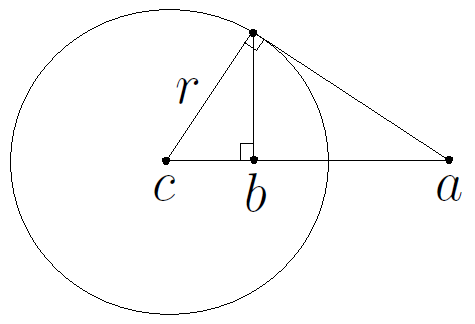
\includegraphics[scale=0.3]{SphericalInversion}
\caption{The inversion $a$ (or $b$) of a point $b$ (or $a$) about a sphere with radius $r$.}
\end{figure}

Using what we know about similar triangles, it is not hard to show that
\begin{equation*}
b=(1-\gamma)c+\gamma a,
\end{equation*}
where $\gamma$ is given by
\begin{equation*}
\gamma = \left(\frac{r}{|c-a|}\right)^2=\left(\frac{|c-b|}{r}\right)^2.
\end{equation*}
Letting $p:\R^n\to\V$ be defined as it is in equation \eqref{equ_p_conformal}, we find that
\begin{equation*}
\sigma p(a)\sigma^{-1}=-\gamma^{-1}p(b),
\end{equation*}
where $\sigma$ is given by
\begin{equation*}
\sigma = p(c)-\frac{1}{2}r^2\nvai.
\end{equation*}
The vector $\sigma$, therefore, is an example of a preservative versor.  In fact, it is
not hard to show that every versor of the conformal model is preservative.
Letting $V$ be a versor of the conformal model, simply show that $Vp(x)V^{-1}$ is null,
and therefore of the form $\lambda p(y)$.

\begin{defn}\label{def_preservative_versor_induced_func}
For any preservative versor $V\in\G$, we let $V_p:\R^n\to\R^n$ denote
the function induced by $V$ through $p:\R^n\to\V$ as mapping any point $x\in\R^n$
to the corresponding point $y\in\R^n$ satisfying equation \eqref{equ_vpv_p}.
\end{defn}

Notice that $V_p$ in Definition~\ref{def_preservative_versor_induced_func} is a well defined function.

\begin{lem}\label{lem_when_V_p_is_a_bijection}
If $V\in\G$ is a preservative versor, then $V^{-1}$ is a preservative versor
if and only if $V_p$ is one-to-one and onto $\R^n$.
\end{lem}
\begin{proof}
Given that $V$ is a preservative versor, we first show that
if $V^{-1}$ is a preservative versor, then $V_p$ is one-to-one and onto $\R^n$.

For any $y\in V_p(\R^n)$, let $x_1,x_2\in\R^n$ be a pair of points,
and $\gamma_1,\gamma_2\in\R$ be a pair of non-zero scalars
such that $V^{-1}p(x_1)V=\gamma_1p(y)$ and $V^{-1}p(x_2)V=\gamma_2p(y)$.
Rearranging these equations, we find that $Vp(y)V^{-1}=\gamma_1^{-1}p(x_1)$
and $Vp(y)V^{-1}=\gamma_2^{-1}p(x_2)$.  It then follows, by the
preservative property of $V^{-1}$, that
$\gamma_1=\gamma_2$ and $x_1=x_2$.

Now for any $y\in\R^n$, we know, by the preservative property of $V^{-1}$,
that there exists a non-zero $\gamma\in\R$ and a point $x\in\R^n$ such that
$Vp(y)V^{-1}=\gamma p(x)$.  Rearranging, we find that
\begin{equation}
V^{-1}p(x)V=\gamma^{-1}p(y)\implies V_p(x)=y.
\end{equation}

Given that $V$ is a preservative versor, we now show that
if $V_p$ is one-to-one and onto $\R^n$, then $V^{-1}$ is a preservative versor.

Rearranging equation \eqref{equ_vpv_p}, we get
\begin{equation}\label{equ_vpv_p_rearranged}
Vp(y)V^{-1} = \gamma^{-1}p(x).
\end{equation}
Now simply realize that since $V_p$ is one-to-one and onto $\R^n$, for every $y\in\R^n$,
there exists a unique pair of a point $x\in\R^n$ and a non-zero scalar $\gamma\in\R$ such that
equation \eqref{equ_vpv_p_rearranged} holds.
\end{proof}

Notice that if a versor $V\in\G$ is preservative, and $V^{-1}$ is preservative,
then $V_p^{-1}=(V^{-1})_p$.

\begin{thm}\label{thm_how_preservative_versor_transforms}
For any blade $A\in\B$,
if $V\in\G$ is a preservative versor, and $V^{-1}$ is also preservative, then
\begin{equation}
\gh(VAV^{-1}) = V_p^{-1}(\gh(A)) = \{x\in\R^n|V_p(x)\in\gh(A)\}.
\end{equation}
\end{thm}
\begin{proof}
If $x\in\gh(VAV^{-1})$, then there exists a blade $B\in\B$
such that $VAV^{-1}=B\wedge p(x)$.  Then, for a non-zero scalar $\gamma\in\R$,
we have
\begin{equation}
A=V^{-1}BV\wedge\gamma p(V_p(x))\implies V_p(x)\in\gh(A).
\end{equation}

If $V_p(x)\in\gh(A)$, then there exists a blade $B\in\B$
such that $A = B\wedge p(V_p(x))$.  Then, for a non-zero scalar $\gamma\in\R$,
we have, by Lemma~\ref{lem_when_V_p_is_a_bijection},
\begin{equation}
VAV^{-1}=VBV^{-1}\wedge\gamma p(x)\implies x\in\gh(VAV^{-1}).
\end{equation}

In each direction, note the use of Lemma~\ref{lem_desired_partial_blade_factorization}.
\end{proof}

Theorem~\ref{thm_how_preservative_versor_transforms} shows us that the
problem of determining how a given preservative
versor $V\in\G$ transforms a geometric set reduces to the problem of determining
how the function $V_p:\R^n\to\R^n$ transform space, provided $V^{-1}$ is preservative too.

\begin{cor}
If $V\in\G$ is a preservative versor, and $V^{-1}$ is preservative, and $A,B\in\B$ are any pair
of blades such that $\gh(A)=\gh(B)$, then
\begin{equation}
\gh(VAV^{-1})=\gh(VBV^{-1}).
\end{equation}
\end{cor}
\begin{proof}
By Theorem~\ref{thm_how_preservative_versor_transforms}, we simply notice that
\begin{equation}
\gh(VAV^{-1})=V_p^{-1}(\gh(A))=V_p^{-1}(\gh(B))=\gh(VBV^{-1}).
\end{equation}
\end{proof}

\begin{cor}
If $V\in\G$ is a preservative versor, and $V^{-1}$ is preservative,
and $A\in\B$ is a blade such that $\gh(A)=\emptyset$, then
\begin{equation}
\gh(VAV^{-1})=\emptyset.
\end{equation}
\end{cor}
\begin{proof}
By Theorem~\ref{thm_how_preservative_versor_transforms}, we simply notice that
\begin{equation}
\gh(VAV^{-1})=V_p^{-1}(\gh(A))=V_p^{-1}(\emptyset)=\emptyset.
\end{equation}
\end{proof}

%\begin{lem}
%If for every irreducible blade $A\in\B$ of grade 1, we have $|\gh(A)|=1$, then
%for every preservative versor $V\in\G$, the function $V_p$ is one-to-one.
%\end{lem}
%\begin{proof}
%For any $y\in V_p(\R^n)$, let $x_1,x_2\in\R^n$ be a pair of points,
%and $\gamma_1,\gamma_2\in\R$ be a pair of non-zero scalars
%such that $V^{-1}p(x_1)V=\gamma_1p(y)$ and $V^{-1}p(x_2)V=\gamma_2p(y)$.
%It then follows that
%\begin{equation}
%p(x_1)=\frac{\gamma_1}{\gamma_2}p(x_2) \implies p(x_1)\wedge p(x_2)=0 \implies x_1\in\gh(p(x_2))=\{x_2\}.
%\end{equation}
%\end{proof}

\subsection{Reduction}

Interestingly, while Theorem~\ref{thm_geo_set_rep} showed the existence and uniqueness of irreducible blades,
the problem of fully reducing a given blade has no obvious solution.  To illustrate this, let us assume, for this section,
that $\G$ has a euclidean signature.
(There are now no null-vectors in $\G$.)  Under this assumption, consider the following algorithm which
attempts to fully reduce a given blade $A$.

\begin{algorithmic}
\Function{Reduce}{$A$}
	\State $B\gets 1$
	\State $x\gets$\Call{FindAnyPoint}{$A$}
	\If{$p(x)\wedge A=0$}
		\State $B\gets p(x)\,\wedge\,$\Call{Reduce}{$p(x)\cdot A$}
	\EndIf
	\State\Return $B$
\EndFunction
\end{algorithmic}
Here, the function ``FindAnyPoint'' finds, (perhaps using methods of calculus), and returns any point in $\gh(A)$.
If no such point can be found, any point is returned.

Working in a geometric algebra with a euclidean signature, if for the $r$-blade $A$, we have $p(x)\wedge A=0$,
there exists an $(r-1)$-blade $C\in\B$ such that $p(x)\cdot C=0$ and $A=p(x)\wedge C=p(x)C$.  (The
Gram-Schmidt orthogonalization process is always applicable in euclidean geometric algebras.)
It then follows that
\begin{equation}
p(x)\cdot A = \langle p(x)^2 C\rangle_{r-1}=|p(x)|^2 C.
\end{equation}

The algorithm ``Reduce'' above is simply a factorization algorithm that is looking for
vector factors of a specific form.  By design, it may terminate before the blade is fully factored;
in which case, a reduction $B$ of the blade $A$ may have been found.  Though $B$, the returned blade,
is clearly irreducible, it is not clear whether $B$ directly represents the same geometric set that is
directly represented by $A$.  The algorithm can only guarantee
that $\gh(B)\subseteq\gh(A)$, because we can't be sure that $B$ is the largest irreducible subspace of $A$.

A correct algorithm would be as follows.

\begin{algorithmic}
\Function{Reduce}{$A$}
	\State $B\gets 1$
	\State $x\gets$\Call{FindPoint}{$A$, $B$}
	\While{$p(x)\wedge A=0$ {\bf and} $p(x)\wedge B\neq 0$}
		\State $B\gets B\wedge p(x)$
		\State $x\gets$\Call{FindPoint}{$A$, $B$}
	\EndWhile
	\State\Return $B$
\EndFunction
\end{algorithmic}
Here, the function ``FindPoint'' finds a point that is in $\gh(A)$, but not in $\gh(B)$.  (The function is allowed to make the assumption that
$B$ is a subspace of $A$.)  If no such point can be
found, any point is returned.  It is not immediately clear, however, how one might go about implementing such a function.
In an attempt to do so, one might first find the blade $C$ for which $A=B\wedge C$, then look for a point $x\in\gh(C)$.
If one is found, that point can be returned.  If one is not found, the search must find a point $x\in\gh(A)$ for which the
the vector $p(x)$, when written as a linear combination of the vectors in any factorization of $B$ and $C$, non-trivially uses
the vector factors of $C$.

\subsection{Examples}

\subsubsection{Composition/Decomposition}

Here it may be worth giving an example that illustrates an application of Theorem~\ref{thm_geo_set_rep}.
We begin by letting $\G$ be a geometric algebra generated by a 10-dimensional euclidean vector space $\V$, letting $n=3$, and then defining
$p:\R^n\to\V$ as
\begin{align}
p(x) = e_0
 &+ x_1e_1 + x_2e_2 + x_3e_3 \nonumber\\
 &+ x_2x_3e_4 + x_1x_3e_5 + x_1x_2e_6 \nonumber\\
 &+ x_1^2e_7 + x_2^2e_8 + e_3^2e_9,\label{equ_p_quadric}
\end{align}
where here we're using the notation\footnote{This notation is overloaded.  In some cases, $x_i$ denotes a member
of a sequence of points, while in others, $x_i$ denotes a component of $x$ as a vector.  The meaning of $x_i$ should
always be clear from context.} $x_i=x\cdot e_i$.  (Notice that here we're letting $\R^n$ be
a 3-dimensional subspace of $\V$, and that for all $x\in\R^3$, $p(x)\neq 0$.)  Having done this,
we turn our attention to an equation for the $e_3$-axis-aligned elliptical cylinder, given by
\begin{equation}
\frac{(x_1-h)^2}{a^2}+\frac{(x_2-k)^2}{b^2}-1=0.
\end{equation}
Factoring $p(x)$ out of this equation in terms of the inner product, we get $p(x)\cdot E=0$,
where $E$ is given by
\begin{equation}
E = \left(\frac{h^2}{a^2}+\frac{k^2}{b^2}-1\right)e_0-2\frac{h}{a^2}e_1-2\frac{k}{b^2}e_2+\frac{1}{a^2}e_7+\frac{1}{b^2}e_8.
\end{equation}
It follows that for a non-zero scalar $\alpha\in\R$, $\alpha E\wedge e_3$ is a canonical form for a dually represented ellipse in the $x_3=0$ plane.
Given a blade $A\in\B$ known to dually represent such a shape in this plane, one would hope to decompose it using the following equations.
\begin{align}
h &= (-e_{31}\cdot A)(2e_{37}\cdot A)^{-1}\label{equ_decompose_first} \\
k &= (-e_{32}\cdot A)(2e_{38}\cdot A)^{-1} \\
\alpha &= (h^2e_{37}+k^2e_{38}-e_{30})\cdot A \\
a^2 &= \alpha(e_{37}\cdot A)^{-1} \\
b^2 &= \alpha(e_{38}\cdot A)^{-1}\label{equ_decompose_last}
\end{align}
(Here, $e_{ijk\dots}=e_ie_je_k\dots$.)
The problem with this idea is that it can be easily shown that $E\wedge e_3$ is a reducible blade; and therefore,
the blades $A$ and $E\wedge e_3$ may not be scalar multiples of one another.
To see why, consider the following equation which expresses the form of $p(x)$ for all points in the $x_3=0$ plane.
\begin{equation}\label{equ_p_form_in_x3_eq_z_plane}
p(x_1e_1+x_2e_2)=e_0 + x_1e_1 + x_2e_2 + x_1x_2e_6 + x_1^2e_7 + x_2^2e_8
\end{equation}
Now notice that an upper-bound on the dimension of a vector space that can be spanned by vectors
of this form is clearly 6 as there are only 6 components on the right-hand side of equation \eqref{equ_p_form_in_x3_eq_z_plane}.
But $E\wedge e_3$ is a 2-blade, making its dual a blade of grade $10-2=8>6$.  It follows that there is no set of
8 points $\{x_i\}_{i=1}^8$ on an ellipse for which $\bigwedge_{i=1}^8 p(x_i)\neq 0$.

To illustrate the case that $A$ is not a scalar multiple of $E\wedge e_3$, consider the solution set
to the equation
\begin{equation}
x_1^2 + x_2^2 - (x_3+1)^2\tan\frac{\pi}{4}=0,
\end{equation}
which gives us a canonical surface partially submerged below the $x_3=0$ plane.
Factoring $p(x)$ out of this equation in terms of the inner product, we get $p(x)\cdot C=0$,
where $C$ is given by
\begin{equation}
C = -e_0 - 2e_3 + e_7 + e_8 - e_9.
\end{equation}
Letting $A=C\wedge e_3$ and seeing that $A$ dually represents a circle in the $x_3=0$ plane, let us consider
the problem of decomposing it into its characteristic parts using equations
\eqref{equ_decompose_first} through \eqref{equ_decompose_last}.
Again, it is easy to see that $AI$ is reducible, and further, that it is no scalar multiple of $E\wedge e_3$.
(Note that $I=e_{0123456789}$.)
Fully reducing $AI$, we get the 5-blade $C'$, given by
\begin{equation}
C' = e_{01267} - e_{01268} + e_{12678} = e_{126}\wedge(e_0+e_8)\wedge(e_8-e_7).
\end{equation}
To prove that this really is the full reduction of our blade $AI$, Theorem~\ref{thm_geo_set_rep}
allows that we verify just two conditions.
First, that $\gh(C')=\gh(AI)$, which can be done with symbolic computation software.
And secondly, that $C'$ is irreducible, which follows immediately by construction and Lemma~\ref{lem_factorization_of_irreducible_blades}.
The blade $C'$ was constructed by choosing 5 points on the circle, and then using a software
program to expand the outer product of the image of those points under $p:\R^n\to\V$.

Then, by Theorem~\ref{thm_geo_set_rep} once more, this blade $C'$ must be a subspace
of $(E\wedge e_3)I$.  Sure enough, we have
\begin{equation}
(e_{459}\wedge C')I = \alpha E\wedge e_3,
\end{equation}
and we get $\alpha=1$ with the unit circle in the $x_3=0$ plane, centered at origin.
(That is, $h=k=0$ and $a=b=1$.)

The lesson learned here is that we can always make use of a canonical form if we first
fully reduce the blade we wish to decompose.\footnote{Unfortunately, as noted
earlier, the problem of fully reducing a blade remains as yet unresolved.}  Sometimes, however, this is undesirable.
For example, if we were to fully reduce a blade directly representative of a tangent
point in the conformal model, then we would be left with an ordinary point and lose the tangential information.
This brings up the point that a blade may embed within it more information than just the geometric
set that it represents dually or directly.

\subsubsection{Point-Fitting}

Given equation \eqref{equ_p_quadric}, here we investigate conditions upon
which a set of points $\{x_i\}$ has the property that $\bigwedge_i p(x_i)\neq 0$.
It is already immediately clear that, in the case of equation \eqref{equ_p_quadric},
if $\{x_i\}$ is a linearly independent set, then so is the set $\{p(x_i)\}$, but we
can do a little better than this, as the following lemma shows.
\begin{lem}\label{lma_non_co_planar}
If the points in a given set of $j>2$ points $\{x_i\}_{i=1}^j$ are non-co-planar for a hyper-plane of
dimension $j-2$, then the set of vectors $\{p(x_i)\}_{i=1}^j$, (see equation \eqref{equ_p_quadric}),
is linearly independent.
\end{lem}
\begin{proof}
Proving the contrapositive of the lemma, let $\{\lambda_i\}_{i=1}^j$ be
a set of scalars in $\R$, not all zero, such that $0=\sum_{i=1}^j\lambda_i p(x_i)$.
It follows that $0=\sum_{i=1}^j\lambda_i(e_0+x_i)$ and therefore
$0=\sum_{i=1}^j\lambda_i$ and $0=\sum_{i=1}^j\lambda_i x_i$.
Now realize that if there exists an integer $a\in[1,j]$ such that $\lambda_a\neq 0$,
then there must exist an integer $b\in[1,j]-\{a\}$ such that $\lambda_b\neq 0$.
Without loss of generality, let $a=j$ so that $1\leq b\leq j-1$, and write
\begin{equation*}
0 = \sum_{i=1}^j\lambda_ix_i = \sum_{i=1}^{j-1}\lambda_ix_i - \left(\sum_{i=1}^{j-1}\lambda_i\right)x_j = -\sum_{i=1}^{j-1}\lambda_i(x_j-x_i),
\end{equation*}
which shows that the set of vectors $\{x_j-x_i\}_{i=1}^{j-1}$ is linearly dependent.
It now follows that the $(j-1)$-dimensional simplex determined by the points in $\{x_i\}_{i=1}^j$
has no $(j-1)$-dimensional hyper-volume.  That is,
\begin{equation*}
0 = \frac{1}{(j-1)!}\bigwedge_{i=1}^{j-1}(x_j-x_i).
\end{equation*}
But this can only be if the $j$ points are co-planar for a hyper-plane of dimension $j-2$.
\end{proof}
Note that the condition of Lemma~\ref{lma_non_co_planar} is certainly sufficient, but
not entirely necessary.  Nothing about the non-linear terms of $p:\R^n\to\V$ were ever
taken into account.  A condition on $\{x_i\}$, whose satisfaction is had if and only if the
set $\{p(x_i)\}$ is linearly independent, is not easy to find.

\section{Closing}

In closing, a few remarks might be made.  First, there are surely more results to be had
about geometric sets in an abstract setting.  The advantage to seeking out such
results is that they will be applicable to any model of geometry we invent
in geometric algebra that uses blades to represent subsets of $\R^n$ as we have
done in this paper.  On the other hand,
we may find that more advanced models of geometry use multi-vectors generally
for such a purpose, or something other than geometric algebra altogether.
As shown in \cite{Parkin13}, multivectors homogeneous of a grade $s$ are
natural representatives of $s$-degree polynomial surfaces.  Perhaps it is
worth looking at geometric algebras that are generated by the linear space
of all $s$-vectors taken from another geometric algebra.

Lastly, there has been a
lofty and naive expectation among geometric algebraists (the present author not included)
that a reformulation of algebraic geometry in terms of geometric algebra would somehow enrich the subject
in ways beyond the current capabilities of abstract algebra.  However, even with a limited understanding
of algebraic geometry, it is abundantly clear that this notion is absurd.  Nevertheless,
geometric algebra should not be discounted; for it may bring some meaningful
contributions to the study of solution sets of algebraic equations.

An end will now be made by saying that, as with any paper, a great deal of care has been taken to insure
the accuracy of every
equation and every claim.  Nevertheless, in my weakness and lack of mathematical maturity,
if you've found a mistake, (or two, or more), hopefully they can be easily
corrected without invalidating the main results of the paper.

\begin{thebibliography}{9}

\bibitem{Dorst07}
L. Dorst, et. al.,
\emph{Geometric Algebra for Computer Science}.
Morgan Kaufmann, 1st edition, 2007.

\bibitem{Fontijne10}
D. Fontijne, et. al.,
\emph{Efficient algorithms for factorization and join of blades}.
Geometric Algebra Computing, Springer London, pp. 457-476, 2010.

\bibitem{Gallian06}
J. Gallian,
\emph{Contemporary Abstract Algebra}.
Houghton Milffin, 6th edition, 2006.

\bibitem{Garrity13}
T. Garrity, et. al.,
\emph{Algebraic Geometry, A Problem Solving Approach}.
American Mathematical Society, Institute for Advanced Study,
Volume 66, 2013.

\bibitem{Hestenes01}
D. Hestenes,
\emph{Old Wine in New Bottles: A new algebraic framework for computational geometry}.
Advances in Geometric Algebra with Applications in Science and Engineering,
Birkhauser Boston, pp. 3-17, 2001.

\bibitem{Lasenby04}
A. Lasenby, et. al.,
\emph{A Covariant Approach to Geometry using Geometric Algebra}.
University of Cambridge, Department of Engineering, 2004.

\bibitem{Parkin13}
S. Parkin,
\emph{The Mother Minkowski Algebra Of Order $M$}.
Advances in Applied Clifford Algebras, Volume 24, Issue 1, pp 193-203, 2013.

\end{thebibliography}

\end{document}